\documentclass[letter]{article}
\usepackage{tutorial}
\usepackage[OT1]{fontenc}

% ------------------------------------------------------------------------
\usepackage{graphicx}
\usepackage{subfigure}
\usepackage{epsfig}
\usepackage{psfrag}
% used to write c++ code/algorithms
\usepackage{listings}
\usepackage{fancyvrb}

%\psdraft

% hyperref stuff
\usepackage{hyperref}
\hypersetup{
  pdftitle={Getting started with CGAL Polyhedron},
  pdfauthor={INRIA Geometrica},
  pdfsubject={A tutorial for CGAL},
  pdfkeywords={},
  pdfpagemode=UseThumbs,
  baseurl={http://www.cgal.org},
  colorlinks=true,
  linkcolor=black,
  anchorcolor=black,
  citecolor=black,
  filecolor=black,
  menucolor=black,
  pagecolor=black,
  urlcolor=blue,
  bookmarksopen=false,}
% end hyperref stuff

\lstset{language=C++, basicstyle=\scriptsize}

\graphicspath{{figs/}}
\def\figurename{Figure}
\def\tablename{Tableau}
\newcommand{\italic}[1]{\emph{#1}} 

% ------------------------------------------------------------------------
\newcommand\IL{{\itshape left}}
\newcommand\IR{{\itshape right}}
\newcommand\IM{{\itshape middle}}
\newcommand\IT{{\itshape top}}
\newcommand\IB{{\itshape bottom}}

% ------------------------------------------------------------------------
\newcommand{\CodeFmt}[1]{{\small\texttt{#1}}}

\def\kernel{\CodeFmt{Kernel}}

\def\cgalpoly{\CodeFmt{CGAL::Polyhedron\_3}}
\def\poly{\CodeFmt{Polyhedron\_3}}
\def\polytrait{\CodeFmt{PolyhedronTraits\_3}}
\def\polyitem{\CodeFmt{PolyhedronItems\_3}}
\def\polybuilder{\CodeFmt{Polyhedron\_incremental\_builder\_3}}

\def\cgalhds{\CodeFmt{CGAL::HalfedgeDS}}
\def\hds{\CodeFmt{HalfedgeDS}}
\def\hdsitem{\CodeFmt{PolyhedronItems}}

% L.K. -------------------------------------------------------------------
\newcommand{\CC}{C\raise.08ex\hbox{\texttt{++}}}
\newcommand{\openmesh}{\textsc{OpenMesh}}
\newcommand{\opensg}{\textsc{OpenSG}}
\newcommand{\cgal}{\textsc{Cgal}}
\newcommand{\stl}{\textsc{Stl}}


% =========================================================================
\begin{document}

% TITLE
% ------------------------------------------------------------------------
\date{}
\title{{\LARGE {\sffamily\bfseries A Tutorial on CGAL Polyhedron Meshing}}}
% pierre: other suggestions for the title?
%  Mesh Processing with CGAL Polyhedron
%  Algorithms on Meshes with CGAL Polyhedron
%  Getting started with CGAL Polyhedron
% ?

\author{\small
\sffamily Le-Jeng Shiue\footnote{SurfLab, University of Florida}
\and \small
\sffamily Pierre Alliez\footnote{GEOMETRICA, INRIA Sophia-Antipolis}
\and \small
\sffamily Radu Ursu\footnote{GEOMETRICA, INRIA Sophia-Antipolis}
\and \small
\sffamily Lutz Kettner\footnote{MPII, Saarbr\"ucken}}
\maketitle

\thispagestyle{empty}

% ABSTRACT
% ------------------------------------------------------------------------
\abstract{
We will present a tutorial on the CGAL polyhedron data structure
assuming familiarity with the C++ template mechanism and the 
key concepts of the generic programming. The tutorial is 
organized around a meshing application. 
It starts with a polyhedron viewer for a customized polyhedron.
The polyhedron viewer demonstrates the basic functionalities 
of the \cgalpoly\ and some extend functionalities such as file I/O, 
mesh superimposition, and trackball manipulation.
The tutorial also shows how to implement subdivision algorithms
in three different approaches. These approaches are proposed with 
increasing level of sophistication and abstraction. The 
simplest approach uses the atomic operators 
of the combinatorial modifications to implement 
$\sqrt{3}$ subdivision scheme. 
A second approach overloads the modifier, with the help 
of the incremental builder, to implement 
quad-triangle subdivision. The third approach abstracts 
the geometry operations from the refinements.
This approach specializes a subdivision with
template geometry rules. Catmull-Clark, Loop and Doo-Sabin
subdivisions are illustrated based on the third approach. 
}
%%\vskip 3mm

\begin{center} 
  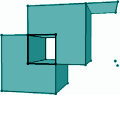
\includegraphics[width=12.0cm]{figs/teaser}\\
{\scriptsize Demo application running on Windows. A polygon mesh is 
   subdivided using the quad-triangle subdivision scheme.}
\end{center}

\subsection*{Generic Mesh Data Structure}
Polyhedron data structures based on the concept of
halfedges have been very successful for the design
of general algorithms on meshes. 
Although making a preliminary version of a halfedge-based mesh data
structure is as a fairly simple task and is often proposed as a
programming exercise, the time has come where we should not write our
own mesh data structure from scratch anymore. With the emerging of
the generic programming in C++, a set of reusable library
components for graphics modeling and geometry processing are demanded
by researchers and developers. \emph{Extensible algorithm} models based on
a \emph{robust, efficient and customizable polyhedron 
data structure} will certainly speed up
the research as well as the development cycle, and benefit the 
community of the graphics modeling and geometry processing.  

Most of mesh algorithms employ a customized 
halfedge data structures and most of the customizations 
are specialized by customizing the primitive data, 
which are the vertex positions, the facet normals or other 
algorithmic flags. \cgalpoly\ encapsulates a generic
design of the halfedge data structure allowing users
customize the \poly\ with the template parameters of
the geometry primitives. There are several advantages
that employing the \poly\ as the core data structure
of a meshing application: \\
\indent $\bullet$ The \poly\ is a \emph{generic} data structure.\\
\indent $\bullet$ The \poly\ is a \emph{robust} and \emph{optimized} 
data structure.\\
\indent $\bullet$ A complete set of the geometry entities and predications 
is provided within CGAL.\\
\indent $\bullet$ CGAL is standardized following the C++ STL.

\subsection*{Demo Application for Meshing}
We have designed and implemented a meshing application
based on the \cgalpoly . This program provides a
polyhedron viewer that supports following functionalities:\\
\indent $\bullet$ File I/O,\\
\indent $\bullet$ polyhedron rendering,\\ 
\indent $\bullet$ and trackball manipulation.\\
In addition to these build-in functions, the viewer 
is accompanied with a set of subdivision algorithms
that generate smooth polyhedron surfaces from
a coarse polyhedron. \emph{The tutorial  
instructs the readers through the design and the implementation 
of the polyhedron viewer and the subdivisions}. The first part of the 
tutorial highlights the design and implementation issues 
related to the \poly\ of the viewer. The second part
of the tutorial explains how to implement 
the connectivity and geometry operations of the 
subdivision algorithms. The source codes are going to 
be published with the releasing of the tutorial.

\subsection*{Tutorial Outlines}
\subsubsection*{Polyhedron Viewer}
The tutorial starts with demonstrating
how to implement a simple viewer based on the default
configuration of the \cgalpoly . This simple viewer 
demonstrates some basic functionalities of the \cgalpoly\ such as
\emph{modifier} and \emph{incremental builder} for initialization and 
the mesh traversal, i.e. the \emph{iterators} and the \emph{circulators},
for rendering or mesh exporting. Based on this simple
viewer, we then show the readers how to
\emph{customize the \poly} to support certain functionalities. 
An enriched polyhedron is proposed with the primitives 
specialized with algorithmic flags. This enriched polyhedron
is used as the core data structure of our meshing application.
We then show how to interact with a customized \poly . 
The extended primitives are employed to support the superimposition of the 
input mesh on the subdivided surfaces. A trackball function
of the enriched polyhedron is also demonstrated in the tutorial.

\subsubsection*{Subdivision Algorithms}
The second part of the tutorial focuses on the design and 
the implementation of the subdivision algorithms.
In addition to the importance in surface modeling,
we choose subdivision algorithms to demonstrate
both the \emph{topology operation} (refinement) and the 
\emph{geometry operations} (smoothing). The topology and the geometry
operations are the two basic operations required by
most geometry algorithms. Our implementations of the subdivisions 
are designed to be a separated library that accept 
any generic \poly\ as the input polyhedron (not just the 
enriched polyhedron we used in the polyhedron viewer). The key to implement
a subdivision algorithm is to support the refinement, 
i.e.\ the connectivity modifications.
Two approaches are first introduced to support the refinement:
the \emph{atomic operators of the combinatorial modifications}
(operator scheme) and the \emph{modifier mechanism} (modifier scheme).
The operator scheme reconfigures
the connectivity with a combination of several combinatorial 
operators. The $\sqrt{3}$ subdivision is used to
demonstrate this scheme. Though simple and efficient 
in some refinements, e.g.\ $\sqrt{3}$ 
subdivision, the correct combination of the operators is 
hard to find for some refinements, 
e.g.\ Doo-Sabin subdivision. The modifier scheme
solves the problem by letting the programmers 
create their own combinatorial operators
using the polyhedron incremental builder.
The Quad-Triangle subdivision is used to demonstrate this scheme.

\subsubsection*{Generic Subdivisions}
Subdivisions can be represented
as a combination of a refinement and a set of smoothing
rules. Based on this observation, our third approach 
generalizes the subdivision by abstracting the smoothing rules
from the refinement. The refinement is designed as a \emph{host 
function} that accepts a \emph{policy class} supporting the 
smoothing rules. A subdivision function is then a 
legal combination of the refinement and the smoothing rules.
For example, the Catmull-Clark subdivision can be declared
as: 
\begin{lstlisting}
void CatmullClark_subdivision(Polyhedron& p) {    
  quadralize_polyhedron<CatmullClark_rule<Polyhedron>>(p);  
}
\end{lstlisting}
The \lstinline!quadralize_polyhedron<>! represents the refinement 
(host function) and the \lstinline!CatmullClark_rule<>! supports
the geometry rules (policy).
This approach offers a convenient way to specialize a subdivision 
with the \emph{template smoothing rules}.
Catmull-Clark, Loop and Doo-Sabin subdivisions are 
illustrated based on this approach. 

\subsection*{Intended Audience}
The intended audience of the tutorial are researchers, 
developers or students in the graphics community developing 
algorithms around meshes. Experience in advanced C++
design (i.e.\ generic programming using templates) and
knowledge of the halfedge data structure and 
subdivisions are prerequisites. 

\end{document}
